\documentclass{article}

\usepackage{graphicx}
\usepackage{tikz}
\usepackage{tikzsymbols}
\usetikzlibrary{calc,patterns,shapes.geometric}
\pagestyle{empty}
\usepackage[margin=0pt]{geometry}
\geometry{papersize={14in,12in}}

\def\centerarc[#1](#2)(#3:#4:#5){\draw[#1] ($(#2)+({#5*cos(#3)},{#5*sin(#3)})$) arc (#3:#4:#5);}

\begin{document}
	\begin{figure}
		\centering
		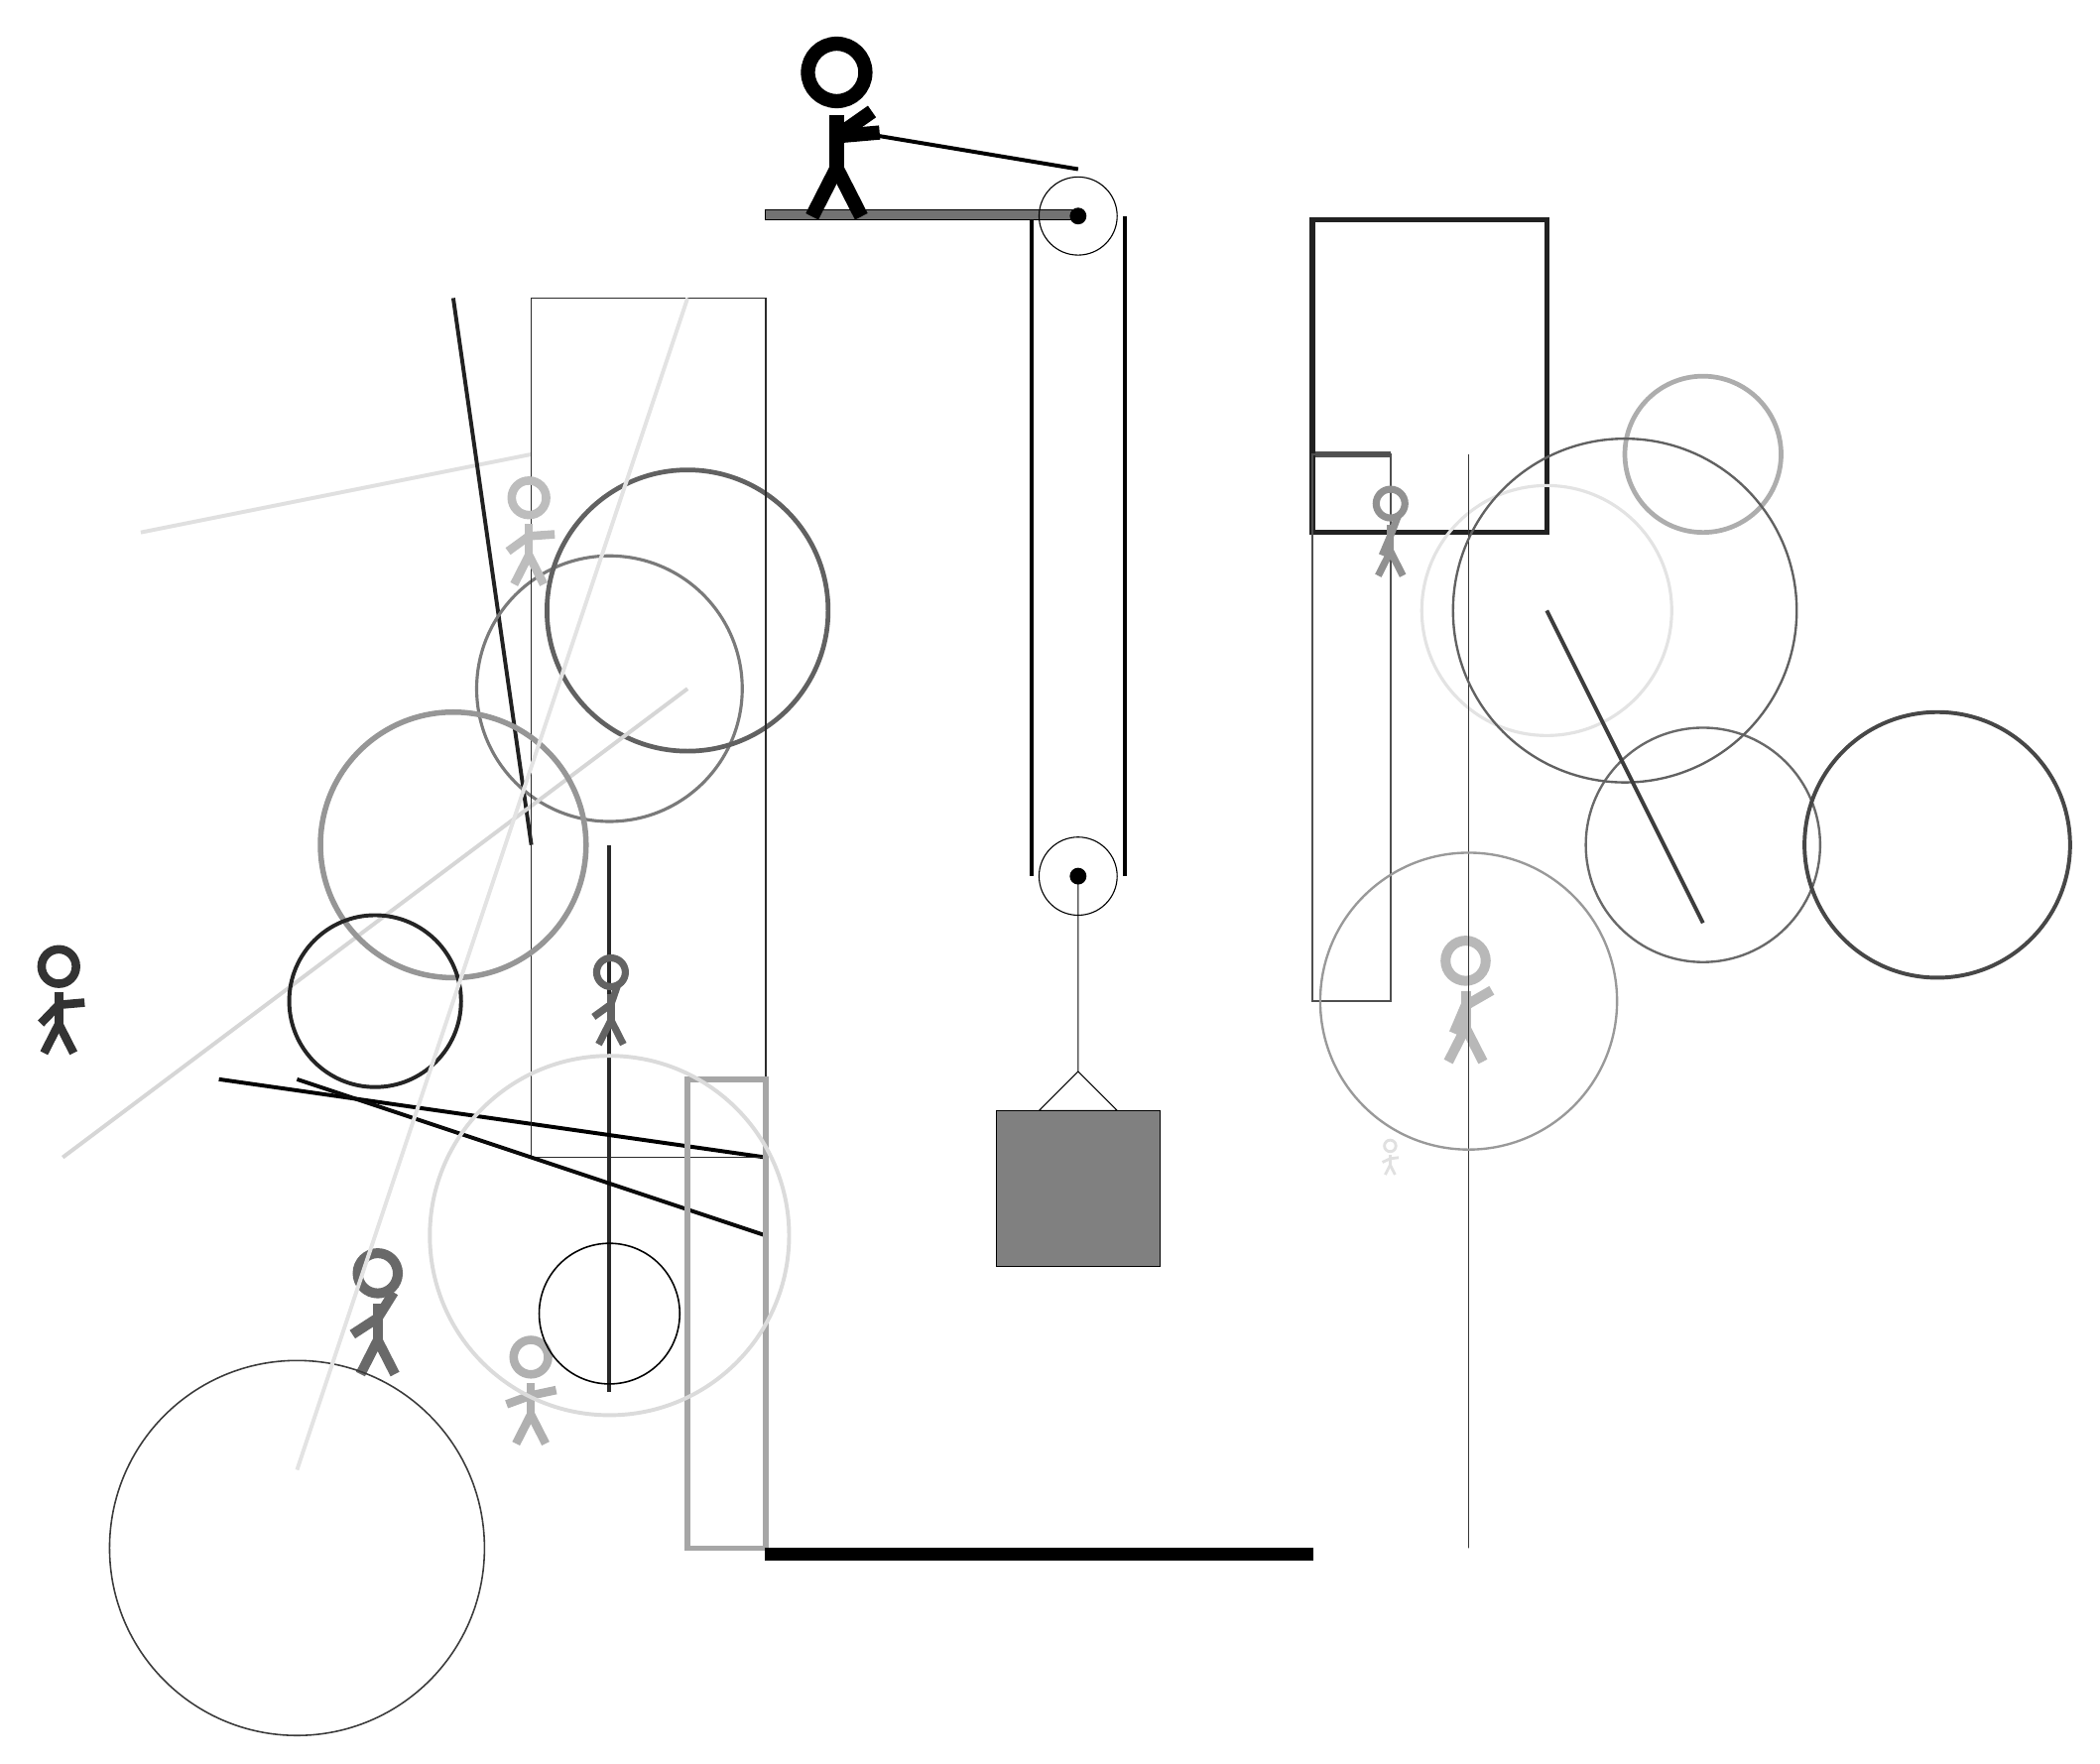
\begin{tikzpicture}
			%%%%% START %%%%%
			
			\draw[fill=black!55] (-2, 14) rectangle (2, 14.125);
			
			\draw[line width=0.7mm, color=black!68] (6, 11) rectangle (5, 11);
			
			\draw[line width=0.5mm, color=black!12](-5, 11) -- (-10, 10);
			\draw[line width=0.5mm, color=black!87](-5, 6) -- (-6, 13);
			\draw[line width=0.5mm, color=black!84](-4, 6) -- (-4, -1);
			\draw[line width=0.7mm, color=black!87] (5, 14) rectangle (8, 10);
			
			\draw [line width=0.5mm, color=black!78](12, 3) circle (0.0);
			\draw [line width=0.4mm, color=black!52](-4, 8) circle (1.7);
			\draw[line width=0.5mm, color=black!100](-2, 2) -- (-9, 3);
			\node[line width=0.3mm, color=black!80] at (-11, 4) {\Strichmaxerl[6][46][5]};
			
			\draw [line width=0.3mm, color=black!59](10, 6) circle (1.5);
			\draw [line width=0.5mm, color=black!72](13, 6) circle (1.7);
			\node[line width=0.5mm, color=black!28] at (7, 4) {\Strichmaxerl[7][67][30]};
			\node[line width=0.5mm, color=black!59] at (-7, 0) {\Strichmaxerl[7][33][58]};
			
			\node[line width=0.2mm, color=black!31] at (-5, -1) {\Strichmaxerl[6][20][12]};
			\draw [line width=0.6mm, color=black!62](-3, 9) circle (1.8);
			\draw [line width=0.6mm, color=black!32](10, 11) circle (1.0);
			
			\draw[line width=0.5mm, color=black!16](-3, 8) -- (-11, 2);
			\draw [line width=0.4mm, color=black!11](8, 9) circle (1.6);
			\draw[line width=0.2mm, color=black!83] (-2, 2) rectangle (-5, 13);
			
			\draw [line width=0.7mm, color=black!41](-6, 6) circle (1.7);
			\draw [line width=0.5mm, color=black!86](-7, 4) circle (1.1);
			
			\draw [line width=0.2mm, color=black!77](-8, -3) circle (2.4);
			\draw [line width=0.2mm, color=black!100](-4, 0) circle (0.9);
			\draw[line width=0.5mm, color=black!96](-2, 1) -- (-8, 3);
			\node[line width=0.5mm, color=black!26] at (-5, 10) {\Strichmaxerl[6][36][4]};
			\draw[line width=0.2mm, color=black!69] (6, 11) rectangle (5, 4);
			
			\draw[line width=0.7mm, color=black!35] (-2, -3) rectangle (-3, 3);
			\node[line width=0.7mm, color=black!43] at (6, 10) {\Strichmaxerl[5][67][69]};
			\draw[line width=0.2mm, color=black!79] (7, -3) rectangle (7, 11);
			
			\draw [line width=0.5mm, color=black!14](-4, 1) circle (2.3);
			\draw [line width=0.3mm, color=black!62](9, 9) circle (2.2);
			
			\draw[line width=0.5mm, color=black!11](-3, 13) -- (-8, -2);
			\draw [line width=0.3mm, color=black!40](7, 4) circle (1.9);
			\node[line width=0.4mm, color=black!61] at (-4, 4) {\Strichmaxerl[5][36][71]};
			\node[line width=0.6mm, color=black!12] at (6, 2) {\Strichmaxerl[2][25][7]};
			\draw[line width=0.5mm, color=black!76](8, 9) -- (10, 5);
			
			\draw (2, 5.6) circle (0.5);
			\draw[fill=black] (2, 5.6) circle (0.1);
			
			\draw (2, 14.05) circle (0.5);
			\draw[fill=black] (2, 14.05) circle (0.1);
			
			\draw (2, 5.6) -- (2, 3.1) -- (1.5, 2.6) -- (2.5, 2.6) -- (2, 3.1);
			\draw[fill=black!50] (0.95, 2.6) rectangle (3.05, 0.6);
			
			\draw[line width=0.5mm] (1.4, 14) -- (1.4, 5.6);
			\centerarc[line width=0.5mm](2, 5.6)(180:360:0.6);
			\draw[line width=0.5mm](2.6, 5.6) -- (2.6, 14.05);
			\centerarc[line width=0.5mm](2, 14.05)(0:90:0.6);
			\draw[line width=0.5mm](2, 14.65) -- (-1, 15.15);
			
			\node at (-1, 15.15) {\Strichmaxerl[10][-175][35]};
			
			\draw[fill=black] (-2, -3) rectangle (5, -3.15);
			
			%%%%% END %%%%%
		\end{tikzpicture}
	\end{figure}	
\end{document}